\achapter{1}{Sets}\label{sec:sets}


\vspace*{-17 pt}
\framebox{
\parbox{\dimexpr\linewidth-3\fboxsep-3\fboxrule}
{\begin{fqs}
\item What is a set?
\item What is a subset of a set?
\item What is the union of two sets? How do we define the union of an arbitrary collection of sets?
\item What is the intersection of two sets? How do we define the intersection of an arbitrary collection of sets?
\item What is the complement of a set? 
\item What is the Cartesian product of sets?
\end{fqs}}}

\vspace*{13 pt}

\csection{Introduction} 

At its most basic level topology deals with sets and how we can deform sets into other sets. So to start our study of topology, we begin with sets. Much of this material should be familiar, but some might be new.  The first issue for us to settle on is as precise a definition of ``set" as possible.

\begin{pa} \label{pa:sets} Suppose we try to define a set to be a collection of elements. So, by definition, the elements are the objects contained in the set. We use the symbol $\in$ to denote that an object is an element of a set. So $\notin$ means an object is not in the set -- if $x$ is an object in a set $S$ we write $x \in S$, and if $x$ is not an object in a set $S$ we write $x \notin S$. We write sets using set brackets. For example, the set $\{a,b,c\}$ is the set whose elements are the symbols $a$, $b$, and $c$. We can also include in the set notation conditions on elements of the set. For example, $\{x \in \R : x > 0\}$ is the set of positive real numbers. We typically use capital letters to denote sets. Some familiar examples of sets are $\R$, the set of real numbers; $\Q$, the set of rational numbers; and $\Z$, the set of integers. Sets can also contain sets as elements. For example, the power set of a set  $S$ is the set of subsets of $S$. So the power set of $S = \{1,2\}$ is the set $\{\emptyset, \{1\}, \{2\}, \{1,2\}\}$. (We will define subsets and the empty set later in this activity).   

\be
\item Consider the following ``set" $S$, which is a collection of objects:
	\[S = \{A \text{ is a set} \mid A \notin A\}.\]
	That is, $S$ is the collection of sets that do not have themselves as elements. 

Given any object $x$, either $x \in S$ or $x \notin S$. 
	\ba
	\item Is $S$ an element of $S$? Explain.

	\item Is it the case that $S \notin S$? Explain. 
	
	\item Based on your responses to parts (a) and (b), explain why our current concept of a set as a collection of elements is not a good one.  

	\ea

\item Assume that we have a working definition of a set. In this part of the activity we define a subset of a set. The notation we will use is $A \subset S$ if $A$ is a subset of $S$ that is not equal to $S$, and $A \subseteq S$ if $A$ is a subset of $S$ that could be the entire set $S$. We will also say that $A$ is \emph{contained} in $S$ if $A$ is a subset of $S$, and call the relation $A \subset S$ (or $A \subseteq S$) a \emph{containment}.

	\ba
	\item How should we define a subset of a set? Give a specific example of a set and two examples of subsets of that set.
	
	\item If $A$ is a set, is $A$ a subset of $A$? Explain.

	\item What is the empty set $\emptyset$? If $A$ is a set, is $\emptyset$ a subset of $A$? explain.

	\ea

\ee

\end{pa}

\begin{comment}

\ActivitySolution
\be
\item Let $S = \{A \text{ is a set} \mid A \notin A\}$. 
	\ba
	\item If $S \in S$, then $S$ does not contain itself as an element. But then $S$ cannot be in $S$, so this is not possible.

	\item If $S \notin S$, then $S$ must contain itself as an element. But this contradicts the fact that $S \notin S$. 

	\item Our current definition of a set leads to a paradox -- a set with an element that is neither in the set nor not in the set. 
	
	\ea

\item
	\ba
	\item A subset $U$ of a set $S$ is a collection of elements of $S$. That is, $U$ is a subset of $S$ if $x \in S$ whenever $x \in U$. For example, if $S = \{1,2,3,4\}$, then $\{1,2\}$ and $\{1,3,4\}$ are subsets of $S$. 
	
	\item Since every element of $A$ is also an element of $A$, by our definition it is the case that $A$ is a subset of $A$. 
	
	\item The empty set is the set that contains no elements. Since $\emptyset$ contains no elements, by default every element of $\emptyset$ is an element of any other set. So $\emptyset$ is a subset of every set. 
	
	\ea	
\ee


\end{comment}


\csection{The Basic Idea of Topology}

If you like geometry, you will probably like topology. Geometry is the study of objects with certain attributes (e.g., shape and size), while topology is more general than geometry. In topology, we aren't concerned about the attributes (shape and size) of an object, only about those characteristics that don't change when we transform the object in different ways (any way that doesn't involve tearing or poking holes the object).  There are lots of really interesting theorems in topology -- for example, the Hairy Ball Theorem which states that if you have a ball with hair all over it (think of a tribble from Star Trek -- if that isn't too old of a reference), it is impossible to comb the hairs continuously and have all the hairs lay flat. Some hair must be sticking straight up! 

\begin{activity} \label{act:rubber_sheet} ~
\ba
\item Take a pipe cleaner, a rubber band, or a piece of string and make a square from it. You are allowed to change the square by moving parts of the square without breaking it or lifting it off the surface it is on. To which of the following shapes can you transform your square? Explain. 
\begin{center}
(i.) a circle \qquad (ii.) the letter \texttt{S} \qquad (iii.) a five point star {\raisebox{-1mm}{\resizebox{!}{0.2in}{\includegraphics{star.eps}}}} \qquad (iv.) the letter \texttt{D} 
\end{center}


\item Now take some play-doh (if you don't have any play-doh, just use your imagination). Use the play-doh (or your imagination) to determine which of the following shape can be transformed into others without breaking or making holes.
\begin{center}
(i.) a filled sphere  \qquad (ii.) a doughnut \qquad (iii.) a bowl \qquad (iv.) a coffee mug with handle
\end{center}

\ea

\end{activity}

\begin{comment}

\ActivitySolution
\ba
\item 
	\begin{enumerate}[i.]  
	\item We can take the unit circle and fix the points where the circle intersects the coordinate axes. Push the remaining points on the circle toward the square in a radial manner. This deforms the circle onto the square.
	\item In order to make the letter \texttt{S}, we would have to cut the circle. Since this is not allowed, we cannot deform the circle to the letter $\texttt{S}$.
	\item Think of the circle as being inscribed inside the star. Then push out the portions of the circle that are not on the star toward the arms. This deforms the circle onto the star.
	\item Consider the unit circle as our circle. Project the left half of the circle onto the $y$-axis. This deforms the circle onto the letter \texttt{D}.	
	\end{enumerate}

\item  Smash down the top half of the sphere onto the bottom half. This makes a bowl. To make a doughnut or a coffee mug with a handle, we would have to punch a hole in the sphere. So the sphere and the bowl can be deformed onto one another, but neither can be deformed into a doughnut or a coffee mug.  However, we can deform a coffee mug into a doughnut (see \url{https://en.wikipedia.org/wiki/File:Mug_and_Torus_morph.gif}) for an animation. The process involves molding the mug part around the handle until the result is a doughnut. This process can be reversed, so a coffee mug and a doughnut can be deformed into each other.  

\ea


\end{comment}

This idea of transforming one set into another as we explored in Activity \ref{act:rubber_sheet} is formally done with functions. As we progress through this subject, we will need to have more rigorous definitions of functions and sets. We begin with sets and discuss functions in Section \ref{sec:functions}. 

\csection{Intervals}

We will begin with one of the most basic type of set we will encounter -- intervals. The open intervals will be important as they will form a basis for the standard topology on $\R$. We are likely familiar with intervals from algebra and calculus, sets like $(0,1)$, $[2,3)$. To really understand intervals, we will need a rigorous definition.

\begin{definition} A subset $I$ of $\R$ is an \textbf{interval}\index{interval} if for all $a$, $b$, and $c$ in $\R$ (allowing for $a$ or $b$ to be $\pm \infty$) with $a < c < b$, if $a$ and $b$ are in $I$, then $c$ is in $I$. 
\end{definition}

With this definition, the set of all real numbers $x$ satisfying $0 < x < 1$ is an interval that we denote by $(0,1)$ (it is important to understand the context -- we also use the notation $(0,1)$ to denote an ordered pair). The general notation we use for intervals is the following: 
\begin{itemize}
\item $(a,b) = \{t \in \R \mid a < t < b\}$  ($a$ or $b$ could be $\pm \infty$)
\item $[a,b) = \{t \in \R \mid a \leq t < b\}$  ($b$ could be $\pm \infty$)
\item $(a,b] = \{t \in \R \mid a < t \leq b\}$  ($a$ could be $\pm \infty$)
\item $[a,b] = \{t \in \R \mid a \leq t \leq b\}$.
\end{itemize}

In this notation, $\R = (-\infty, \infty)$. Intervals of the form $(a,b)$ are called \emph{open} intervals, intervals of the form $[a,b]$ are called \emph{closed} intervals, and intervals of the form $[a,b)$ or $(a,b]$ are \emph{half-open} (or \emph{half-closed}) intervals. The reason for this terminology should become more clear as we introduce open and closed sets later. 

Note that nothing in the definition indicates that we must have $a < b$ in the interval notation. This implies that $(1,1)$ is an interval. Since there are no real numbers larger than $1$ and less than $1$,  $\emptyset = (1,1)$ is an interval. We could also have an interval of the form $[a,a]$ where $a$ is any real number. This means that $\{a\} = [a,a]$, and any single point set is an interval. The intervals $\emptyset$ and $[a,a]$ for any real number $a$ are called \emph{degenerate} intervals.  

One last note about intervals. Some require that $a$ be less than $b$ in the definition of an interval, with the result that there are no degenerate intervals. This is a matter of debate that we won't get into. In almost all of our work, we will consider only non-degenerate intervals so this won't be an issue for us. 


\csection{Unions, Intersections, and Complements of Sets}

In mathematics, the collection of points that make up a string or a blob of play-doh as in Activity \ref{act:rubber_sheet} is represented as a set. Topology is then the study of these sets and what properties of the sets don't change when transformations are applied to the sets. To study topology we will need a solid understanding of sets and different operations on sets. 

What we saw in Preview Activity \ref{pa:sets} is what is called a \emph{paradox}. Our original attempt to define a set led to an impossible situation since both $S \in S$ and $S \notin S$ lead to contradictions. This paradox is called \emph{Russell's paradox} after Bertrand Russell, although it was apparently known before Russell. The moral of the story is that we need to be careful when making definitions. A set might seem like a simple object, and in our experience usually is, but formally defining a set can be problematic. As a result, we won't state a formal definition, but rather take a set\index{set} to be a collection of objects that doesn't lead to a paradox. The objects are called the elements of the set. (In axiomatic set theory, a set is taken to be an undefined primitive -- much as a point is undefined in Euclidean geometry.)  

In order to effectively work with sets, we need to have an understanding what it means for two sets to be equal.

\begin{activity} \label{act:set_equality} ~
	\ba
	\item What should it mean for two sets to be equal? If $A$ and $B$ are sets, how do we prove that $A = B$? (This is question that requires discussion, which is different than a question that only asks for a computation or an example. Activities throughout this text will ask both types of questions.)

	\item Let $A = \{x \in \R \mid x < 2\}$ and $B = \{x \in \R \mid x-1 < 1\}$. Is $A=B$? If yes, prove your answer. If no, prove any containment that you can.
	
	\item Let $A = \{n \in \Z \mid 2 \text{ divides } n\}$ and $B = \{n \in \Z \mid 4 \text{ divides } (n-2)\}$. Is $A=B$? If yes, prove your answer. If no, prove any containment that you can.


	\item Let $A = \{n \in \Z \mid n \text{ is odd}\}$ and $B = \{n \in \Z \mid 4 \text{ divides } (n-1)  \text{ or } 4 \text{ divides } (n-3)\}$. Is $A=B$? If yes, prove your answer. If no, prove any containment that you can.
	
	\ea

\end{activity}

\begin{comment}

\ActivitySolution

\ba
\item Two sets $A$ and $B$ are equal if $A \subseteq B$ and $B \subseteq A$. So to prove that two sets $A$ and $B$ are equal, we choose an arbitrary element $a$ in $A$ and show that $a \in B$, and then choose an arbitrary element $b \in B$ and show that $b \in A$. 

\item First we show that $A \subseteq B$. Let $a \in A$. Then $a < 2$. This implies that $a - 1 < 2-1 = 1$, so $a \in B$. Thus, $A \subseteq B$. Now assume that $b \in B$. Then $b-1 < 1$. But this implies that $(b-1)+1 < 1+1$ or $b < 2$. Thus $b \in A$ and $B \subseteq A$. The two containments demonstrate that $A = B$. 

\item We show that $B \subset A$, but $A \neq B$. Let $b \in B$. Then $4$ divides $b-2$. It follows that there exists an integer $k$ such that $b-2 = 4k$. So $b = 2+4k = 2(1+2k)$ and $2$ divides $b$. We conclude that $b \in A$ and $B \subseteq A$. However, $2$ divides $4$, but $4$ does not divide $4-2$. So $A$ is not a subset of $B$. 

\item We will prove that $A = B$. Let $a \in A$. Then $a$ is odd, so there exists an integer $q$ such that $a = 2q+1$. Now $q$ is either even or odd, and we consider the cases. If $q$ is even, then $q = 2p$ for some integer $p$. In this case $a = 2(2p) + 1 = 4p+1$ and $4$ divides $a-1$. If $q$ is odd, then $q =2p+1$ for some integer $p$. Then we have $a = 2(2p+1)+1 = 4p+3$ and $4$ divides $a-3$. Thus, $a \in B$ and $A \subseteq B$. Now let $b \in B$. Then $4$ divides $b-1$ or $4$ divides $b-3$. If $4$ divides $b-1$, then $b-1 = 4k$ for some integer $k$. But then $b = 1+4k = 1+2(2k)$ for some integer $k$, which shows that $b$ is odd. If $4$ divides $b-3$, then $b = 4k+3$ for some integer $k$. It follows that $b = 3+4k = 1+2(1+2k)$ for some integer $k$, which again shows that $b$ is odd. Thus $b \in A$ and $B \subseteq A$. The two containments demonstrate that $A = B$. 

\ea

\end{comment}

Once we have the notion of a set, we can build new sets from existing ones. For example, we define the union, intersection, set difference, and complement of a set as follows.

\begin{itemize}
\item The \textbf{union}\index{set!union} of sets $A$ and $B$ is the set $A \cup B$ defined as 
\[A \cup B = \{x \mid x \in A \text{ or } x \in B\}.\]
\item The \textbf{intersection}\index{set!intersection} of sets $A$ and $B$ is the set $A \cap B$ defined as
\[A \cap B = \{x \mid x \in A \text{ and } x \in B\}.\]
\item Let $A$ and $B$ be sets. The \textbf{set difference}\index{set difference} $A \setminus B$ is the set 
\[A \setminus B = \{a \in A \mid a \notin B\}.\]
\item Let $A$ be a subset of a set $U$. The \textbf{complement}\index{set!complement} of $A$ in $U$ is the set 
	\[U \setminus A = \{x \in U \mid x \notin A\}.\]
The complement of a set $A$ in a set $U$ is also denoted by $C_U(A)$, $C(A)$ (if the set $U$ is understood), $A^c$, or even $U-A$. 
\end{itemize}

We can visualize these sets using Venn diagrams. A Venn diagram is a depiction of sets using geometric figures. For example, if $U$ is a set containing all other sets of interest (we call $U$ the \emph{universal} set), we can represent $U$ as a large container (say a rectangle) with subsets $A$ and $B$ as smaller containers (say circles), and shade the elements in a given set. The Venn diagrams in Figure \ref{F:Venn} depict the sets $A$, $B$, $A \cup B$, $A \cap B$, $A^c$, and $B^c$. 
\begin{figure}[h]
\begin{center}
 \begin{minipage}[th!]{0.2\textwidth}
  	\begin{center}
  	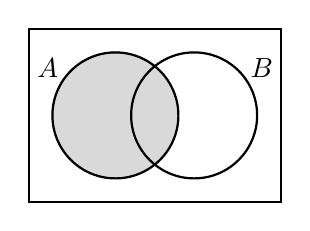
\begin{tikzpicture}[scale=0.4]
		\def\universal{(-4,-2.75) -- (4,-2.75) -- (4,2.75) -- (-4,2.75) -- cycle}		
		\def\firstcircle{(-1.25,0) circle (2cm)}
		\def\secondcircle{(1.25,0) circle (2cm)}
		\draw[fill=gray!30] \firstcircle;
		\draw[thick] \firstcircle;
		\draw[thick] \secondcircle;
		\draw[thick] \universal;
		\node at (-3.4,1.5) {$A$};
		\node at (3.4,1.5) {$B$};
	\end{tikzpicture}\\
	$A$
	\end{center}
  \end{minipage}
  \hspace{1.0cm}
   \begin{minipage}[th!]{0.2\textwidth}
  	\begin{center}
  	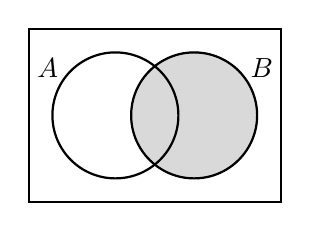
\begin{tikzpicture}[scale=0.4]
		\def\universal{(-4,-2.75) -- (4,-2.75) -- (4,2.75) -- (-4,2.75) -- cycle}		
		\def\firstcircle{(-1.25,0) circle (2cm)}
		\def\secondcircle{(1.25,0) circle (2cm)}
		\draw[fill=gray!30] \secondcircle;
		\draw[thick] \firstcircle;
		\draw[thick] \secondcircle;
		\draw[thick] \universal;
		\node at (-3.4,1.5) {$A$};
		\node at (3.4,1.5) {$B$};
	\end{tikzpicture}\\
	$B$
	\end{center}
  \end{minipage}
    \hspace{1.0cm}
   \begin{minipage}[th!]{0.2\textwidth}
  	\begin{center}
  	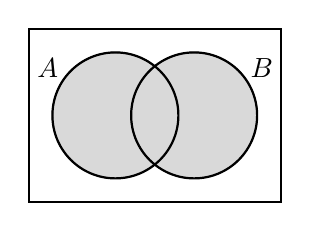
\begin{tikzpicture}[scale=0.4]
		\def\universal{(-4,-2.75) -- (4,-2.75) -- (4,2.75) -- (-4,2.75) -- cycle}		
		\def\firstcircle{(-1.25,0) circle (2cm)}
		\def\secondcircle{(1.25,0) circle (2cm)}
		\draw[fill=gray!30] \firstcircle;
		\draw[fill=gray!30] \secondcircle;
		\draw[thick] \firstcircle;
		\draw[thick] \secondcircle;
		\draw[thick] \universal;
		\node at (-3.4,1.5) {$A$};
		\node at (3.4,1.5) {$B$};
	\end{tikzpicture}\\
	$A \cup B$
	\end{center}
  \end{minipage}

\vspace{0.5cm}

   \begin{minipage}[th!]{0.2\textwidth}
  	\begin{center}
  	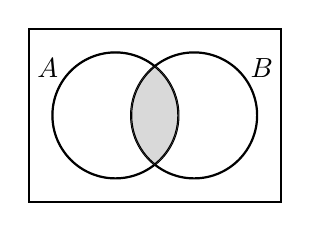
\begin{tikzpicture}[scale=0.4]
		\def\universal{(-4,-2.75) -- (4,-2.75) -- (4,2.75) -- (-4,2.75) -- cycle}		
		\def\firstcircle{(-1.25,0) circle (2cm)}
		\def\secondcircle{(1.25,0) circle (2cm)}
		\draw[thick] \firstcircle;
		\draw[thick] \secondcircle;
		\draw[thick] \universal;
		\node at (-3.4,1.5) {$A$};
		\node at (3.4,1.5) {$B$};
		\draw[clip] \firstcircle;
		\draw[clip] \secondcircle;
		\fill[gray!30] (0,0) circle (2cm);
		\draw[thick] \firstcircle;
		\draw[thick] \secondcircle;
	\end{tikzpicture}\\
	$A \cap B$
	\end{center}
  \end{minipage}
\hspace{1.0cm}  
 \begin{minipage}[th!]{0.2\textwidth}
  	\begin{center}
  	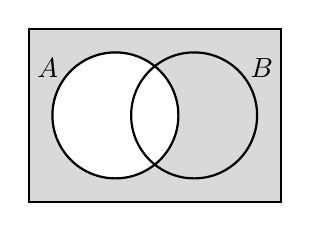
\begin{tikzpicture}[scale=0.4]
		\def\universal{(-4,-2.75) -- (4,-2.75) -- (4,2.75) -- (-4,2.75) -- cycle}		
		\def\firstcircle{(-1.25,0) circle (2cm)}
		\def\secondcircle{(1.25,0) circle (2cm)}
		\draw[fill=gray!30] \universal;
		\draw[fill=white] \firstcircle;
		\draw[thick] \firstcircle;
		\draw[thick] \secondcircle;
		\draw[thick] \universal;
		\node at (-3.4,1.5) {$A$};
		\node at (3.4,1.5) {$B$};
	\end{tikzpicture}\\
	$A^c$
	\end{center}
  \end{minipage}
  \hspace{1.0cm}
 \begin{minipage}[th!]{0.2\textwidth}
  	\begin{center}
  	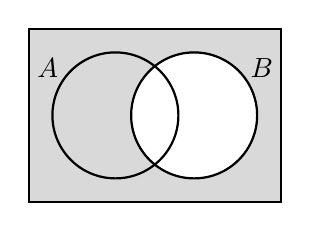
\begin{tikzpicture}[scale=0.4]
		\def\universal{(-4,-2.75) -- (4,-2.75) -- (4,2.75) -- (-4,2.75) -- cycle}		
		\def\firstcircle{(-1.25,0) circle (2cm)}
		\def\secondcircle{(1.25,0) circle (2cm)}
		\draw[fill=gray!30] \universal;
		\draw[fill=white] \secondcircle;
		\draw[thick] \firstcircle;
		\draw[thick] \secondcircle;
		\draw[thick] \universal;
		\node at (-3.4,1.5) {$A$};
		\node at (3.4,1.5) {$B$};
	\end{tikzpicture}\\
	$B^c$
	\end{center}
  \end{minipage}
\caption{Vennn diagrams}
\label{F:Venn}
\end{center}
\end{figure}
 
As we have discussed, to prove that two sets $X$ and $Y$ are equal we prove that each is a subset of the other. The next example provides another illustration of the  idea.

\begin{example} \label{ex:set_eq} Let $A$, $B$, and $C$ be sets. We will prove that $A \cap (B \setminus C) = (A \cap B) \setminus (A \cap C)$. 

To prove this set equality we must prove that $A \cap (B \setminus C) \subseteq (A \cap B) \setminus (A \cap C)$ and $(A \cap B) \setminus (A \cap C) \subseteq A \cap (B \setminus C)$. We start with $A \cap (B \setminus C) \subseteq (A \cap B) \setminus (A \cap C)$.

To prove that $A \cap (B \setminus C) \subseteq (A \cap B) \setminus (A \cap C)$, we need to demonstrate that every element in $A \cap (B \setminus C)$ is also in $(A \cap B) \setminus (A \cap C)$. To do this, we select an arbitrary element in $A \cap (B \setminus C)$ and show that this element is in $(A \cap B) \setminus (A \cap C)$. Let $x \in A \cap (B \setminus C)$. Then $x \in A$ and $x \in B \setminus C$. The fact that $x \in B \setminus C$ implies that $x \in B$ but $x \notin C$. Therefore, $x \in A$ and $x \in B$, but $x \notin C$. This implies that $x \in A$ and $x \in B$, but $x \in A$ and $x \notin C$. So $x \in A$ and $x \in B$, but $x \notin A \cap C$. We conclude that $x \in (A \cap B) \setminus (A \cap C)$. This proves that $A \cap (B \setminus C) \subseteq (A \cap B) \setminus (A \cap C)$.

For the reverse containment, we let $y \in (A \cap B) \setminus (A \cap C)$. So $y \in A \cap B$ but $y \notin A \cap C$. Since $y \in A \cap B$, we know that $y \in A$ and $y \in B$. The fact that $y \notin A \cap C$ means that $y \notin C$. So $y \in A$, $y \in B$, and $y \notin C$.  Thus, $y \in A$ and $y \in B \setminus C$. We conclude that $y \in A \cap (B \setminus C)$, which shows that $(A \cap B) \setminus (A \cap C) \subseteq A \cap (B \setminus C)$. The two containments, $A \cap (B \setminus C) \subseteq (A \cap B) \setminus (A \cap C)$ and $(A \cap B) \setminus (A \cap C) \subseteq A \cap (B \setminus C)$ demonstrate that $A \cap (B \setminus C) = (A \cap B) \setminus (A \cap C)$.

\end{example}

We will use the ideas in Activity \ref{act:set_equality} and Example \ref{ex:set_eq} to prove set equalities throughout this text. The next activity will provide some additional practice. 
 
\begin{activity} \label{act:sets_1} In this activity we work with unions, intersections, and complements of sets. Let $A$ and $B$ be sets. 
	\ba
	\item  Let $A = \{1,2,3,4,5,6\}$ and $B = \{2,4,6,8,10\}$, with $U = \{1,2,3,4,5,6,7,8,9,10\}$. 
		\begin{enumerate}[i.]
		\item Determine the elements in $A \cup B$ and $A \cap B$. What are the elements in $(A \cup B)^c$ and $(A \cap B)^c$?
		
		\item Determine the elements in $A^{c} \cup B^{c}$ and $A^{c} \cap B^{c}$. 

		\end{enumerate}

%	If $U = \{a,b,c,d,e,f,g\}$ and $A = \{c,e,g\}$, what is $U \setminus A$? 
	
	\item Let $A$ and $B$ be arbitrary subsets of a universal set $U$. There are connections between $A$, $B$ and their complements, unions, and intersections. 
		\begin{enumerate}[i.]
		\item Use Venn diagrams to draw $(A \cup B)^c$ and $(A \cap B)^c$.  
		
		\item Use the Venn diagrams and the result of (a) to find and prove a relationship between $A^c$, $B^c$ and $(A \cup B)^c$.

		\item Use the Venn diagrams and the result of (a) to find and prove a relationship between $A^c$, $B^c$ and $(A \cap B)^c$.

		\end{enumerate}
		
	\ea
\end{activity}

\begin{comment}

\ActivitySolution

\ba
\item Let $A = \{1,2,3,4,5,6\}$ and $B = \{2,4,6,8,10\}$, with $U = \{1,2,3,4,5,6,7,8,9,10\}$. 
	\begin{enumerate}[i.]
	
	\item In this example we have 
\[A \cup B = \{1,2,3,4,5,6,8,10\} \ \text{ and } \ A \cap B = \{2,4,6\}.\]

	\item Given $A \cap B$ and $A \cup B$ from part i.,  
\[(A \cap B)^c = \{1,3,5,7,8,9,10\} \ \text{ and } \ A^{c} \cup B^{c} = \{1,3,5,7,8,9,10\}\]
and
\[(A \cup B)^c = \{7,9\} \ \text{ and } \ A^{c} \cap B^{c} = \{7,9\}.\]

	\end{enumerate}
	
%\item In this example we have $U \setminus A = \{a,b,d,f\}$.

\item Venn diagrams illustrating the sets $(A \cup B)^c$ and $(A \cap B)^c$ are shown below.
\begin{center}
 \begin{minipage}[th!]{0.2\textwidth}
  	\begin{center}
  	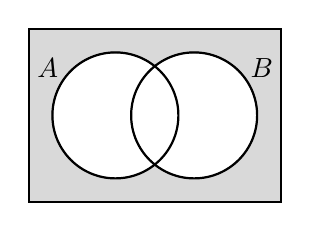
\begin{tikzpicture}[scale=0.4]
		\def\universal{(-4,-2.75) -- (4,-2.75) -- (4,2.75) -- (-4,2.75) -- cycle}		
		\def\firstcircle{(-1.25,0) circle (2cm)}
		\def\secondcircle{(1.25,0) circle (2cm)}
		\draw[fill=gray!30] \universal;
		\draw[fill=white] \firstcircle;
		\draw[fill=white] \secondcircle;
		\draw[thick] \firstcircle;
		\draw[thick] \secondcircle;
		\draw[thick] \universal;
		\node at (-3.4,1.5) {$A$};
		\node at (3.4,1.5) {$B$};
	\end{tikzpicture}\\
	$(A \cup B)^c$
	\end{center}
  \end{minipage}
  \hspace{1.0cm}
 \begin{minipage}[th!]{0.2\textwidth}
  	\begin{center}
  	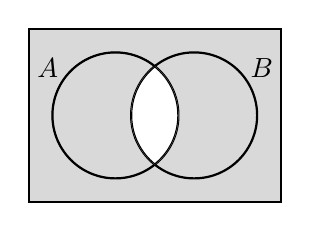
\begin{tikzpicture}[scale=0.4]
		\def\universal{(-4,-2.75) -- (4,-2.75) -- (4,2.75) -- (-4,2.75) -- cycle}		
		\def\firstcircle{(-1.25,0) circle (2cm)}
		\def\secondcircle{(1.25,0) circle (2cm)}
		\draw[fill=gray!30] \universal;	
		\draw[thick] \firstcircle;
		\draw[thick] \secondcircle;
		\draw[thick] \universal;
		\node at (-3.4,1.5) {$A$};
		\node at (3.4,1.5) {$B$};
		\draw[clip] \firstcircle;
		\draw[clip] \secondcircle;
		\fill[white] (0,0) circle (2cm);
		\draw[thick] \firstcircle;
		\draw[thick] \secondcircle;
	\end{tikzpicture}\\
	$(A \cap B)^c$
	\end{center}
  \end{minipage}
\end{center}

	\begin{enumerate}[i.]
	\item The Venn diagrams and (a) indicate that $(A \cup B)^c = A^c \cap B^c$. To prove this statement, start by letting $x \in (A \cup B)^c$. Then $x \notin (A \cup B)$. So $x \notin A$ and $x \notin B$. This means that $x \in A^c$ and $x \in B^c$, which implies that $x \in (A^c \cap B^c)$. We conclude that $(A \cup B)^c \subseteq (A^c \cap B^c)$.
	
Now suppose that $x \in (A^c \cap B^c)$. Then $x \in A^c$ and $x \in B^c$. So $x \notin A$ and $x \notin B$ and $x \notin (A \cup B)$. From this it follows that $x \in (A \cup B)^c$. We conclude that $(A^c \cap B^c) \subseteq (A \cup B)^c$.The two containments demonstrate that $(A \cup B)^c = A^c \cap B^c$.

	\item The Venn diagrams and (a) indicate that $(A \cap B)^c = A^c \cup B^c$.  prove this statement, start by letting $x \in (A \cap B)^c$. Then $x \notin (A \cap B)$. So $x \notin A$ or $x \notin B$. This means that $x \in A^c$ or $x \in B^c$, which implies that $x \in (A^c \cup B^c)$. We conclude that $(A \cap B)^c \subseteq (A^c \cup B^c)$.
	
Now suppose that $x \in (A^c \cup B^c)$. Then $x \in A^c$ or $x \in B^c$. So $x \notin A$ or $x \notin B$, which means $x \notin (A \cap B)$. But this implies that $x \in (A \cap B)^c$. We conclude that $(A^c \cup B^c) \subseteq (A \cap B)^c$.The two containments demonstrate that $(A \cap B)^c = A^c \cup B^c$.

	\end{enumerate}
	
\ea	

\end{comment}

In Activity \ref{act:sets_1} we worked with the union and intersection of two sets. There is no reason to restrict these definitions to only two sets, as the next activity illustrates. 

\begin{activity}  To define an infinite collection of sets we often use what is called an \emph{indexing set}. An indexing set allows us to consider a collection of objects that are in one-to-one correspondence with a set like the positive integers, or even the real numbers. When using an indexing set, we generally make a statement such as ``let $\{A_{\alpha}\}$ for $\alpha \in I$ be a collection of sets indexed by some set $I$". The collection $\{A_{\alpha}\}_{\alpha \in I}$ is called an \emph{indexed family of sets}.\index{indexed family of sets} 

	\ba
	\item The set $I$ could be finite. As an example, let $A_{n} = \{1, 2, 3, \ldots n\}$ for $n$ in the set $I = \{1,2,3, \ldots, 10\}$.
		\begin{enumerate}[i.]
		\item What is $A_5$? What is $A_{8}$? 
		
		\item How many sets are in the indexed family $\{A_n\}_{n \in I}$?
		\end{enumerate}
	
	\item The indexing set can be infinite. For example, let $A_{\alpha} = [0, |\alpha|)$ for $\alpha$ in the set $\R$ (where $[a,b)$ is the interval consisting of the real numbers $x$ such that $a \leq x < b$). In this case, what is $A_5$? What is $A_{\pi}$?  What is $A_{-\frac{2}{3}}$? 
		
	\item We have defined the union and intersection of two sets. The same idea can be extended to define the union and intersection of an indexed collection of sets. 
		\begin{enumerate}[i.]
		\item Recall that if $A$ and $B$ are sets, the intersection $A \cap B$ is the set $\{x \mid x \in A \text{ and } x \in B\}$. How can we extend this definition from two sets to any collection of sets? In other words, how do we \textbf{define} \index{set!arbitrary intersection} 
	\[\bigcap_{\alpha \in I} A_{\alpha}?\]
In the example in (b), what set is $\ds \bigcap_{\alpha \in \R} A_{\alpha}$?
		
	\item Recall that if $A$ and $B$ are sets, the union $A \cup B$ is the set $\{x \mid x \in A \text{ or } x \in B\}$. How can we extend this definition from two sets to any collection of sets? In other words, how do we \textbf{define} \index{set!arbitrary union} 
	\[\bigcup_{\alpha \in I} A_{\alpha}?\]
In the example in (b), what set is $\ds \bigcup_{\alpha \in \R} A_{\alpha}$?
	
	\end{enumerate}
	
	\ea

\end{activity}

\begin{comment}

\ActivitySolution

	\ba
	\item 
		\begin{enumerate}[i.]
		\item In this case we have $A_5 = \{1,2,3,4,5\}$ and $A_{8} = \{1,2,3,4,5,6,7,8\}$. 
		
		\item Since the indexing set has 10 elements there are 10 sets in the indexed collection of sets.
		
		\end{enumerate}
		
	\item In this case we have $A_5 = [0,5)$, $A_{\pi} = [0,\pi)$, and $A_{-\frac{2}{3}} = \left[0, \frac{2}{3}\right)$. 
	
	\begin{enumerate}[i.]

		
	\item We define $\bigcap_{\alpha \in I} A_{\alpha}$ as follows:
	\[\bigcap_{\alpha \in I} A_{\alpha} = \{x \mid x \in A_{\alpha} \text{ for all } \alpha \in I\}.\]
In our example from (b) we claim that $\bigcap_{\alpha \in I} A_{\alpha} = \{0\}$. To prove this statement, we have that $0 \in A_{\alpha}$ for every $\alpha \in \R$ by definition. So $\{0\} \subseteq  \bigcap_{\alpha \in I} A_{\alpha} = \{0\}$. Now we show that $0$ is the only element in $\bigcap_{\alpha \in I} A_{\alpha} = \{0\}$. Let $x$ be a nonzero real number. Then $A_{x/2} = [0, |x|/2)$ does not contain $x$. So $x \notin \bigcap_{\alpha \in I} A_{\alpha} = \{0\}$. We conclude that $\bigcap_{\alpha \in I} A_{\alpha} = \{0\}$.

	
		\item We define $\bigcup_{\alpha \in I} A_{\alpha}$ as follows:
	\[\bigcup_{\alpha \in I} A_{\alpha} = \{x \mid x \in A_{\alpha} \text{ for some } \alpha \in I\}.\]
In our example from (b) we claim that $\bigcup_{\alpha \in I} A_{\alpha} = [0, \infty)$. Since $A_{\alpha} \subset [0, \infty)$ for every $\alpha \in \R$, it follows that $\bigcup_{\alpha \in I} A_{\alpha} \subseteq [0, \infty)$. Now we prove the reverse containment. Let $x \in [0, \infty)$. Then $x \in [0, 2x) = A_{2x}$. Then $x \in \bigcup_{\alpha \in I} A_{\alpha}$ and $[0, \infty) \subseteq \bigcup_{\alpha \in I} A_{\alpha}$. The two containments demonstrate that  $\bigcup_{\alpha \in I} A_{\alpha} = [0, \infty)$.


	\end{enumerate}
	
\ea

\end{comment}

These properties $(A \cap B)^c = A^c \cup B^c$ and $(A \cup B)^c = A^c \cap B^c$ that we learned about in Activity \ref{act:sets_1} are called DeMorgan's Laws. These laws apply to any union or intersection of sets, finite or infinite. The proofs are left Exercise (\ref{ex:DeMorgan}).   

\begin{theorem}[DeMorgan's Laws] Let $\{A_{\alpha}\}$ is a collection of sets indexed by a set $I$ in some universal set $U$. Then 
\begin{enumerate}
\item $\displaystyle \left(\bigcup_{\alpha \in I} A_{\alpha}\right)^c = \bigcap_{\alpha \in I} A_{\alpha}^c$ 
\item $\displaystyle \left(\bigcap_{\alpha \in I} A_{\alpha}\right)^c = \bigcup_{\alpha \in I} A_{\alpha}^c$ 
\end{enumerate}
\end{theorem}

\begin{activity} ~
\ba
\item Verify DeMorgan's Laws in the specific case of $A_{\alpha} = \{1, 2, 3, \ldots \alpha\}$ in $U = \Z$, where $\alpha$ is any element of the indexing set $I = \Z^+$. 

\item Why should the complement of a union be an intersection and why should the complement of an intersection be a union? (Hint: Consider the definitions of unions and intersections.)

\ea

\end{activity}

\begin{comment}

\ActivitySolution 

\ba

\item Let $\Z^- = \{n \in \Z \mid n < 0\}$. First note that $A_{\alpha}^c = \Z^- \cup \{0\} \cup \{\alpha+1, \alpha+2, \ldots\}$. So $\bigcap_{\alpha \in I} A_{\alpha}^c =  \Z^- \cup \{0\}$. Also, $\bigcup_{\alpha \in I} A_{\alpha} = \Z^+$, so $\left(\bigcup_{\alpha \in I} A_{\alpha}\right)^c = \Z^- \cup \{0\}$. 

Since $A_1^c = \Z \setminus \{1\}$, and $1$ is not an element of any $A_{\alpha}^c$, we have $\bigcup_{\alpha \in I} A_{\alpha}^c = \Z \setminus \{1\}$. Since $A_1 = \{1\}$, the only element common to all of the $A_{\alpha}$ is $1$, and $\bigcap_{\alpha \in I} A_{\alpha} = \{1\}$. So $\left(\bigcap_{\alpha \in I} A_{\alpha}\right)^c = \Z \setminus \{1\}$. 

\item Recall that a union is defined as an ``or" statement and an intersection is an ``and" statement. That is $A \cup B$ is the set of elements in $A$ or $B$, and $A \cap B$ is the set of elements in $A$ and $B$.  A complement is a negation, and the negation of ``$A$ or $B$" is ``(not $A$) and (not $B$)". Similarly, the negation of ``$A$ and $B$" is ``(not $A$) or (not $B$)".   

\ea

\end{comment}


\csection{Cartesian Products of Sets}

The final operation on sets that we discuss is the \emph{Cartesian product} (or \emph{cross product}). This is an operation that we have seen before. When we draw the graph of a line $y = mx+b$ in the plane, we plot the points $(x,mx+b)$. These points are ordered pairs of real numbers. We can extend this idea to any sets. 

\begin{definition} Let $A$ and $B$ are sets. The \textbf{Cartesian product}\index{Cartesian product} of $A$ and $B$ is the set 
\[A \times B = \{(a,b) \mid a \in A \text{ and } b \in B\}.\]
\end{definition}

In other words, the Cartesian product of $A$ and $B$ is the set of ordered pairs $(a,b)$ with $a$ coming from $A$ and $b$ coming from $B$. Note that the order is important. 

\begin{activity} ~
	\ba
	\item List all of the elements in $\{\text{red}, \text{blue}\} \times \{\text{car}, \text{truck}, \text{van}\}$. 
	
	\item If $A$ has $m$ elements and $B$ has $n$ elements, how many elements does the set $A \times B$ have? Explain.

	\ea
	
\end{activity}

\begin{comment}

\ActivitySolution

	\ba
	\item The elements are 
	\begin{center} (red,car), (red,truck), (red,van), (blue,car), (blue,truck), (blue,van).\end{center}
	
	\item Any element in $A \times B$ pairs an element of $A$ with an element of $B$. We can choose $n$ elements from $A$ and $m$ from $B$, so the total number of pairings is $nm$. 

	\ea
	

\end{comment}

There is no reason to restrict ourselves to a Cartesian product of just two sets. This is an idea that we have encountered before. The Cartesian product $\R \times \R$ is the standard real plane that we denote as $\R^2$ and the Cartesian product $\R \times \R \times \R$ is the three-dimensional real space denoted as $\R^3$. If we have an indexed collection $\{X_{i}\}$ of sets, with $i$ running through the set of positive integers, then we can define the Cartesian product of the sets $X_{i}$ as the set of infinite sequences $(x_1, x_2, \ldots, x_n, \ldots)$, where $x_i \in X_i$ for each $i \in \Z^+$. We denote this cartesian product as 
\[\Pi_{i \in \Z^+} X_i = \Pi_{i=1}^{\infty} X_i. \]
The capital pi ($\Pi$) is used to represent a product an an analog of the capital sigma ($\Sigma$) that is used to represent a sum. We will study sequences in more detail later. 


To conclude this section we summarize some properties of sets. Many of these properties can be extended to arbitrary collections of sets. Most of the proofs are straightforward. The associative and distributive laws are left for Exercise (\ref{ex:set_props}). 

\newpage
\begin{theorem} Let $A$, $B$, and $C$ be subsets of a universal set $U$. 
\begin{multicols}{2}
\begin{description}
\item[Properties of the Empty Set.]  ~
	\begin{enumerate}[i.]
	\item $A \cap \emptyset = \emptyset$ 
	\item $A \cup \emptyset = A$ 
	\item $A-\emptyset = A$ 
	\item $\emptyset^c = U$
	\end{enumerate}
\item[Properties of the Universal Set.] ~
	\begin{enumerate}[i.]
	\item $A \cap U = A$ 
	\item $A \cup U = U$ 
	\item $A-U = \emptyset$ 
	\item $U^c = \emptyset$  
	\end{enumerate}
\item[Idempotent Laws.] ~
	\begin{enumerate}[i.]
	\item  $A \cap A = A$ 
	\item $A \cup A = A$ 
	\end{enumerate} 
	\vspace{24pt}
\item[Commutative Laws.] ~
	\begin{enumerate}[i.]
	\item $A \cap B  = B \cap A$
	\item $A \cup B = B \cup A$  
	\end{enumerate}
\item[Associative Laws.] ~
	\begin{enumerate}[i.]
	\item $(A \cap B) \cap C = A \cap (B \cap C)$ 
	\item $(A \cup B) \cup C = A \cup (B \cup C)$ 
	\end{enumerate}
\item[Distributive Laws.] ~
	\begin{enumerate}[i.]
	\item $A \cap (B \cup C) = (A \cap B) \cup (A \cap C)$ 
	\item$A \cup (B \cap C) = (A \cup B) \cap (A \cup C)$ 
	\end{enumerate}
\item[Basic Properties.] ~
	\begin{enumerate}[i.]
	\item $\left(A^c\right)^c = A$ 
	\item $A - B = A \cap B^c$ 
	\end{enumerate}
\item[Subsets and Complements.] ~

$A \subseteq B$ \text{ if and only if } $B^c \subseteq A^c$
\end{description}
\end{multicols}
\end{theorem}

\csection{Summary}
Important ideas that we discussed in this section include the following.
\begin{itemize}
\item We can consider a set to be a well-defined collection of elements.
\item A subset of a set is any collection of elements from that set. That is, a subset $S$ of a set $X$ is a set with the property that if $s \in S$, then $s \in X$. 
\item If $X$ and $Y$ are sets, then the union $X \cup Y$ is the set 
\[X \cup Y = \{z \mid z \in X \text{ or } z \in Y\}.\]
The union of an arbitrary collection $\{X_{\alpha}\}$ of sets for $\alpha$ in some indexing set $I$ is the set 
\[\bigcup_{\alpha \in I} X_{\alpha} = \{z \mid z \in X_{\beta} \text{ for some } \beta \in I\}.\]
\item If $X$ and $Y$ are sets, then the intersection $X \cap Y$ is the set 
\[X \cap Y = \{z \mid z \in X \text{ and } z \in Y\}.\]
The intersection of an arbitrary collection $\{X_{\alpha}\}$ of sets for $\alpha$ in some indexing set $I$ is the set 
\[\bigcap_{\alpha \in I} X_{\alpha} = \{z \mid z \in X_{\beta} \text{ for all } \beta \in I\}.\]
\item If $X$ is a set and $A$ is a subset of $X$, then the complement of $A$ in $X$ is the set 
\[A^c = \{x \in X \mid x \notin A\}.\]
\item If $\{X_{i}\}$ is a collection of sets with $i$ in some indexing set $I$, where $I$ is finite or $I$ is the set of positive integers, the Cartesian product $\Pi_{i \in I} X_i$ of the sets $X_{i}$ as the set of all ordered tuples of the form $(x_i)$ where $i \in I$. 
\end{itemize}

\csection{Exercises}

\be

\item Let $A$, $B$, and $C$ be subsets of a set $X$. Express each of the following sets in mathematical notation using the symbols $\cup$, $\cap$, and $\setminus$.
\ba
\item The elements of $X$ that belong to $A$ and $B$, but not $C$.

\item The elements of $X$ that belong to $C$ and either $A$ or $B$.

\item The elements of $X$ that belong to $A$ but not to both $B$ and $C$.

\item The elements of $X$ that belong to none of the sets $A$, $B$, and $C$.

\item The elements of $X$ that fail to belong to at least two of the sets $A$, $B$, and $C$.

\item  The elements of $X$ that fail to belong to at most one of the sets $A$, $B$, and $C$.

\ea

\begin{comment}

\ExerciseSolution

\ba
\item This set $A \cap B$ is the set of elements that belong to both $A$ and $B$. So the set in question is $(A \cap B) \setminus C$. 

\item The set $A \cup B$ is the set of elements belonging to $A$ or $B$. So the set in question is $C \cap (A \cup B)$. 

\item The set of elements that belong to both $B$ and $C$ is $B \cap C$. So the set in question is $A \setminus (B \cap C)$. 

\item We remove the elements of $A \cup B \cup C$ from $X$. So the set in question is $X \setminus (A \cup B \cup C)$. 

\item The set of elements that belong to at least two of the sets $A$, $B$, and $C$ is $(A \cap B) \cup (A \cap C) \cup (B \cap C)$. So the set in question is $X \setminus ((A \cap B) \cup (A \cap C) \cup (B \cap C))$. 

\item  The set of elements that belong to $A$ but not $B$ or $C$ is $A \setminus (B \cup C)$. So the set of elements that belong to exactly one of $A$, $B$, or $C$ is $(A \setminus (B \cup C)) \cup (B \setminus (A \cup C)) \cup (C \setminus (A \cup B))$. The set of elements that belong to none of $A$, $B$, or $C$ is $X \setminus(A \cup B \cup C)$. So the set in question is 
\[(A \setminus (B \cup C)) \cup (B \setminus (A \cup C)) \cup (C \setminus (A \cup B)) \cup (X \setminus(A \cup B \cup C)).\]

\ea

\end{comment}



\item Let $X \subset Y \subset Z$. Prove or disprove.
\ba
\item $C_Y(X) \subset C_Z(X)$.

\item $Z \setminus (Y \setminus X) = X \cup (Z \setminus Y)$. 


\ea

\begin{comment}

\ExerciseSolution

\ba
\item  To prove this containment, we choose an arbitrary element from $C_Y(X)$ and show that the element is also in $C_Z(X)$. Suppose $t \in C_Y(X)$. Then $t \in Y$ but $t \not\in X$. Since $Y \subset Z$, it follows that $t \in Z$. So $t \in Z$ but $t \notin X$. This means $t \in C_Z(X)$. We conclude that $C_Y(X) \subset C_Z(X)$.

\item  To prove $Z \setminus (Y \setminus X) \subseteq X \cup (Z \setminus Y)$, suppose that $t \in Z \setminus (Y \setminus X)$. By definition, $t \in Z$ but $t \notin (Y\setminus X)$. So $t \in X$ or $t \notin Y$. This gives us two possibilities: $t \in Z$ and $t \in X$ or $t \in Z$ and $t \notin Y$. 
\begin{itemize}
\item If $t \in X$ and $t \in Z$, then $X \subset Z$ implies $t \in X$. 
\item If $t \in Z$ and $t \notin Y$, then $t \in Z\setminus Y$. 
\end{itemize}
Thus, we either have $t \in X$ or $t \in Z\setminus Y$. This is the same as saying $t \in X \cup (Z\setminus Y)$. So  $Z \setminus (Y\setminus X) \subseteq X \cup (Z\setminus Y)$.

For the reverse containment, suppose $t \in X \cup (Z\setminus Y)$. Then $t \in X$ or $t \in Z\setminus Y$. We consider the cases.  
\begin{itemize}
\item Suppose $t \in X$. Then $X \subseteq Z$ implies $t \in Z$. The fact that $t \in X$ means that $t \notin Y\setminus X$. Thus, $t \in Z \setminus (Y\setminus X)$.
\item Now suppose that $t \in Z\setminus Y$. Since $Z\setminus Y \subseteq Z$, it follows that $t \in Z$. The facts that $Y\setminus X \subseteq Y$ and $t \notin Y$ also show that $t \notin Y\setminus X$. Thus, $t \in Z \setminus (Y\setminus X)$. 
\end{itemize}
In either case we have $t \in Z \setminus (Y\setminus X)$, and so $X \cup (Z\setminus Y) \subseteq Z \setminus (Y\setminus X)$. The two containments combine to verify that $Z \setminus (Y\setminus X) = X \cup (Z\setminus Y)$.

\ea

\end{comment}

\item \label{ex:set_props} Let $A$ and $B$ be subsets of a universal set $U$. Prove the associative and distributive laws. That is, prove each of the following.
	\ba
	\item $(A \cap B) \cap C = A \cap (B \cap C)$ 
	\item $(A \cup B) \cup C = A \cup (B \cup C)$ 
	\item $A \cap (B \cup C) = (A \cap B) \cup (A \cap C)$ 
	\item$A \cup (B \cap C) = (A \cup B) \cap (A \cup C)$ 
	\ea
	
\begin{comment}

\ExerciseSolution

	\ba
	\item Suppose that $x \in (A \cap B) \cap C$. Then $x \in A \cap B$ and $x \in C$. So $x \in A$ and $x \in B$, and $x \in C$. It follows that $x \in A$ and $x \in B \cap C$, so $x \in  A \cap (B \cap C)$. Thus, $(A \cap B) \cap C \subseteq  A \cap (B \cap C)$. 
	
	Now suppose that $x \in A \cap (B \cap C)$. Then $x \in A$ and $x \in B \cap C$. So $x \in A$, and $x \in B$ and $x \in C$. Thus, $x \in A \cap B$ and $x \in C$ or $x \in (A \cap B) \cap C$. It follows that $A \cap (B \cap C) \subseteq (A \cap B) \cap C$. The two containments show that $(A \cap B) \cap C = A \cap (B \cap C)$.
	
	\item Suppose that $x \in (A \cup B) \cup C$. Then $x \in A \cup B$ or $x \in C$. Thus, $x \in A$ or $x \in B$, or $x \in C$. This means that $x \in A$ or $x \in B \cup C$. It follows that $x \in A \cup (B \cup C)$ and so $(A \cup B) \cup C \subseteq A \cup (B \cup C)$. 
	
	Now suppose that $x \in A \cup (B \cup C)$. Then $x \in A$ or $x \in B \cup C$. From this we can say that $x \in A$, or $x \in B$ or $x \in C$. Then $x \in A \cup B$ or $x \in C$. It follows that that $x \in (A \cup B) \cup C$ and $A \cup (B \cup C) \subseteq (A \cup B) \cup C$. The two containments show that $(A \cup B) \cup C = A \cup (B \cup C)$. 
	
	\item Suppose that $x \in A \cap (B \cup C)$. Then $x \in A$ and $x \in B \cup C$. So $x \in A$ and $x$ is in one of $B$ or $C$. If $x in B$, then $x \in A \cap B$. If $x \in C$, then $x \in A \cap C$. In either case, $x \in (A \cap B) \cup (A \cap C)$. So $A \cap (B \cup C) \subseteq (A \cap B) \cup (A \cap C)$.
	
	Now suppose that $x \in (A \cap B) \cup (A \cap C)$. Then $x \in A \cap B$ or $x \in A \cap C$. If $x \in A \cap B$, then $a \in A$ and $x \in B \subseteq B \cup C$ and so $x \in A \cap (B \cup C)$. Similarly, if $x \in A \cap C$, then $a \in A$ and $x \in C \subseteq B \cup C$ and so $x \in A \cap (B \cup C)$. Thus, $(A \cap B) \cup (A \cap C) \subseteq A \cap (B \cup C)$. The two containments show that $A \cap (B \cup C) = (A \cap B) \cup (A \cap C)$.
	
	\item Suppose that $x \in A \cup (B \cap C)$. Then $x \in A$ or $x \in B \cap C$. If $x \in A$, then $x \in A \cup B$ and $x \in A \cup C$ and $x \in (A \cup B) \cap (A \cup C)$. If $x \in B \cap C$,  then $x \in B \subseteq A \cup B$ and $x \in C \subseteq A \cup C$. So $x \in (A \cup B) \cap (A \cup C)$. We conclude that $A \cup (B \cap C) \subseteq (A \cup B) \cap (A \cup C)$.
	
	Now suppose that $x \in (A \cup B) \cap (A \cup C)$. Then $x \in A \cup B$ and $x \in A \cup C$. If $x \in A$, then $x \in A \cup (B \cap C)$. If $x \notin A$, then $x \in B$ and $x \in C$. So $x \in B \cap C \subseteq A \cup (B \cap C)$. It follows that $(A \cup B) \cap (A \cup C) \subseteq A \cup (B \cap C)$. The two containments show that $A \cup (B \cap C) = (A \cup B) \cap (A \cup C)$.
	
	\ea
	

\end{comment}

\item \label{ex:DeMorgan} Prove DeMorgan's Laws. That is, let $\{A_{\alpha}\}$ be a collection of sets indexed by a set $I$ in some universal set $U$. Prove that 
\begin{enumerate}
\item $\displaystyle \left(\bigcup_{\alpha \in I} A_{\alpha}\right)^c = \bigcap_{\alpha \in I} A_{\alpha}^c$ 
\item $\displaystyle \left(\bigcap_{\alpha \in I} A_{\alpha}\right)^c = \bigcup_{\alpha \in I} A_{\alpha}^c$ 
\end{enumerate}

\begin{comment}

\ExerciseSolution  Let $\{A_{\alpha}\}$ be a collection of sets indexed by a set $I$ in some universal set $U$. First we show that $\displaystyle \left(\bigcup_{\alpha \in I} A_{\alpha}\right)^c = \bigcap_{\alpha \in I} A_{\alpha}^c$. Let $x \in \displaystyle \left(\bigcup_{\alpha \in I} A_{\alpha}\right)^c$. Then $x \in U$ but $x$ cannot be in any of the $A_{\alpha}$. So $x \in A_{\alpha}^c$ for every $\alpha \in I$ and $x \in \displaystyle \bigcap_{\alpha \in I} A_{\alpha}^c$. Thus, $\displaystyle \left(\bigcup_{\alpha \in I} A_{\alpha}\right)^c \subseteq \bigcap_{\alpha \in I} A_{\alpha}^c$. For the reverse containment, suppose $x \in \bigcap_{\alpha \in I} A_{\alpha}^c$. Then $x \in A_{\alpha}^c$ for every $\alpha \in I$. This means that $x \notin A_{\alpha}$ for every $\alpha \in I$. That is, $x \notin \displaystyle \bigcup_{\alpha \in I} A_{\alpha}$. Thus $x \in \displaystyle \left(\bigcup_{\alpha \in I} A_{\alpha}\right)^c$. This shows that $\displaystyle  \bigcap_{\alpha \in I} A_{\alpha}^c \subseteq \left(\bigcup_{\alpha \in I} A_{\alpha}\right)^c$. The two containments demonstrate that $\displaystyle  \bigcap_{\alpha \in I} A_{\alpha}^c = \left(\bigcup_{\alpha \in I} A_{\alpha}\right)^c$.

Now we prove that $\displaystyle \left(\bigcap_{\alpha \in I} A_{\alpha}\right)^c = \bigcup_{\alpha \in I} A_{\alpha}^c$. Let $x \in \displaystyle \left(\bigcap_{\alpha \in I} A_{\alpha}\right)^c$. Then $x \in U$ but $x \notin \displaystyle \bigcap_{\alpha \in I} A_{\alpha}$. So there is a $\beta$ in $I$ such that $x \notin A_{\beta}$. It follows that $x \in A_{\beta}^c$ and so $x \in \displaystyle \bigcup_{\alpha \in I} A_{\alpha}^c$. Thus, $\displaystyle \left(\bigcap_{\alpha \in I} A_{\alpha}\right)^c \subseteq \bigcup_{\alpha \in I} A_{\alpha}^c$. For the reverse containment, assume that $x \in \displaystyle \bigcup_{\alpha \in I} A_{\alpha}^c$. Then $x \in A_{\beta}^c$ for some $\beta \in I$. So $x \notin A_{\beta}$ and $x \notin \displaystyle \bigcap_{\alpha \in I} A_{\alpha}$. We conclude that $x \in \displaystyle \left(\bigcap_{\alpha \in I} A_{\alpha}\right)^c$. Thus, $\displaystyle \bigcup_{\alpha \in I} A_{\alpha}^c \subseteq \left(\bigcap_{\alpha \in I} A_{\alpha}\right)^c$. The two containments demonstrate that $\displaystyle \left(\bigcap_{\alpha \in I} A_{\alpha}\right)^c = \bigcup_{\alpha \in I} A_{\alpha}^c$.

\end{comment}

\item What familiar set is $\emptyset \times A$ for any set $A$? Explain.  

\begin{comment}

\ExerciseSolution If $(x,a) \in \emptyset \times A$, then $x \in \emptyset$. But this is impossible, so there are no elements in $\emptyset \times A$. We conclude that $\emptyset \times A = \emptyset$.

\end{comment}


\item \label{ex:power_set} If $A$ is a set, the power set\index{power set} of $A$, denoted $2^A$ is the collection of all subsets of $A$. 
	\ba
	\item List the elements of $\ds 2^{\{1,2\}}$. 
		
	\item If $A$ is a set with three elements, how many elements are in $2^A$?
		
	\item If $A$ is a set with $n$ elements, make a conjecture about the number of elements in $2^A$. Prove your conjecture?

	\ea
	
\begin{comment}

\ExerciseSolution

	\ba
	\item The subsets of $\{1,2\}$ are $\emptyset$, $\{1\}$, $\{2\}$, and $\{1,2\}$. 
			
	\item There is only one subset of $A$ with no elements, there are $\binom{3}{1} = 3$ subsets of $A$ with one element, there are $\binom{3}{2} = 3$ subsets of $A$ with exactly two elements, and only one subset of $A$ with three elements. So the number of elements in $2^A$, when $A$ has three elements, is
	\[1+3+3+1 = 8.\]
		
	\item We will use the following result about binomial coefficients. For any integer $n \geq 1$, 
\begin{align*}
\binom{n-1}{k-1} + \binom{n-1}{k} &= \frac{(n-1)!}{(k-1)!((n-1)-(k-1))!} + \frac{(n-1)!}{k!(n-1-k)!}  \\
	&= \frac{(n-1)!}{(k-1)!(n-k)!} + \frac{(n-1)!}{k!(n-1-k)!}  \\
	&= \frac{k(n-1)!}{k!(n-k)!} + \frac{(n-k)(n-1)!}{k!(n-k)!}  \\
	&= \frac{k(n-1)!+(n-k)(n-1)!}{k!(n-k)!}  \\
	&= \frac{n(n-1)!}{k!(n-k)!} \\
	&= \frac{n!}{k!(n-k)!} \\
	&= \binom{n}{k}.
\end{align*}
Suppose a set $A$ has $n$ elements. If $k$ is between 0 and $n$, there are $\binom{n}{k}$ subsets of $A$ with exactly $k$ elements. So the number of elements in $2^A$ is 
\begin{equation} \label{eq:binom}
\sum_{k=0}^n \binom{n}{k}.
\end{equation}
We can show via induction that $\sum_{k=0}^n \binom{n}{k} = 2^n$. First notice that $\binom{0}{0} = 1 = 2^0$, so (\ref{eq:binom}) is true if $n=0$. Also, 
\[\binom{1}{0} + \binom{1}{1} = 1+1 = 2 = 2^1,\]
so (\ref{eq:binom}) is true if $n=1$. Now assume that (\ref{eq:binom}) is true for any value of $n$ between 0 and $m$ for some integer $m \geq 1$. Using the facts that $\binom{m+1}{k} = \binom{m}{k-1} + \binom{m}{k}$ established above and $\binom{m+1}{0} = 1 = \binom{m}{0}$ and $\binom{m+1}{m+1} = 1 = \binom{m}{m}$, we have 
\begin{align*}
\sum_{k=0}^{m+1} \binom{m+1}{k} &= \binom{m+1}{0} + \sum_{k=1}^m \binom{m+1}{k} + \binom{m+1}{m+1} \\
	&= \binom{m}{0} + \sum_{k=1}^m \left( \binom{m}{k-1} + \binom{m}{k} \right) + \binom{m}{m} \\
	&= \left( \sum_{k=1}^m \binom{m}{k-1} + \binom{m}{m} \right) + \left( \binom{m}{0} + \sum_{k=1}^m \binom{m}{k} \right) \\
	&= 2 \sum_{k=0}^m  \binom{m}{k} \\
	&= 2\left(2^{m-1}\right) \\
	&= 2^m.
\end{align*}
So the number of elements of $2^A$ is $2^n$ when $A$ has $n$ elements.

	\ea
	
\end{comment}

\item  If $A$ is a set, the power set of $A$, denoted $2^A$ is the collection of all subsets of $A$. (See Exercise (\ref{ex:power_set}).) Critique each of the following statements. Doe the statement make sense or not? If not, explain why and then correct the statement to something that is true (and non-trivial).  
	\ba

	\item If $A$ is a set, then $A \in 2^A$.

	\item If $A$ is a set, then $A \subset 2^A$.

	\item If $A$ is a set, then $\{A\} \subset 2^A$.

	\item If $A$ is a set, then $\emptyset \in 2^A$.

	\item If $A$ is a set, then $\emptyset \subset 2^A$.

	\item If $A$ and $B$ are sets and $A \subseteq B$, then $2^A \subseteq 2^B$. 

	\ea
	
\begin{comment}
	
\ExerciseSolution

\ba

	\item This statement makes sense because $A$ is a subset of $A$. Since $2^A$ is the collection of subsets of $A$, it follows that $A \in 2^A$. 

	\item This statement doesn't make sense. The set $A$ is an element of $2^A$, not a subset. For example, if $A = \{1\}$, then $2^A = \{\emptyset, A\}$, and $A$ is not a subset of $2^A$. The set $\{A\}$ would be a subset of $2^A$. 

	\item  This statement makes sense. The element of the set $\{A\}$ is also an element of $2^A$, so $\{A\} \subset 2^A$.

	\item  This statement makes sense. Recall that $\emptyset$ is a subset of any set, so $\emptyset$ is a subset of $A$. That makes $\emptyset$ an element of $2^A$. 

	\item  This statement makes sense. The empty set is a subset of any set since every element of $\emptyset$ is an element of any set. 
	
	\item  This statement makes sense. Suppose $S \in 2^A$. Then $S$ is a subset of $A$. If $s \in S$, then $s \in A \subseteq B$, so $s \in B$. Thus, $S \subseteq B$. By definition, then, $S \in 2^B$. Therefore, $2^A \subseteq 2^B$. 
	
\ea

\end{comment}
	

\item Let $A$ and $B$ be sets, both of which have at least two distinct members. Prove that there is a subset $W \subset A \times B$ that is not the Cartesian product of a subset of $A$ with a subset of $B$. [Thus, not every subset of a Cartesian product is the Cartesian product of a pair of subsets.]

\begin{comment}


\ExerciseSolution Let $A$ and $B$ be sets, both of which have at least two distinct members. Let $a_1$ and $a_2$ be distinct elements of $A$ and $b_1$, $b_2$ distinct elements of $B$. Let $W = \{(a_1,b_2), (a_2, b_1)\}$. Since the elements of $W$ are ordered pairs of elements, first from $A$, then from $B$, it follows that $W \subset A \times B$. To show that $W$ is not a Cartesian product of a subset of $A$ with a subset of $B$, we proceed by contradiction and suppose that $W = A' \times B'$ for some subsets $A'$ of $A$ and $B'$ of $B$. Since $(a_1, b_2)$ and $(a_2, b_1)$ are in $W$, it follows that $a_1, a_2 \in A'$ and $b_1, b_2 \in B'$. But then $(a_2, b_2) \in A' \times B'$. The fact that $(a_2,b_2) \notin W$ contradicts the fact that $W = A' \times B'$. We conclude that the assumption that led us to this contradiction is false, and that $W$ is is not the Cartesian product of a subset of $A$ with a subset of $B$. 

\end{comment}



\item Let $I$ be the set of real numbers that are greater than $0$. For each $x \in I$, let $A_x$ be the open interval $(0,x)$. Prove that $\bigcap_{x \in I} A_x = \emptyset$, $\bigcup_{x \in I} A_x = I$. For each $x \in I$, let $B_x$ be the closed interval $[0,x]$. Prove that $\bigcap_{x \in I} B_x = \{0\}$, $\bigcup_{x \in I} B_x = I \cup \{0\}$.

\begin{comment}

\ExerciseSolution Let $I$ be the set of real numbers that are greater than $0$. For each $x \in I$, let $A_x$ be the open interval $(0,x)$. We first prove that $\bigcap_{x \in I} A_x = \emptyset$ by proving the containment in each direction. 

Since $\emptyset$ is a subset of any set, we know that $\emptyset \subseteq \bigcap_{x \in I} A_x$. So to prove the equality we only need to demonstrate the containment $\bigcap_{x \in I} A_x \subseteq \emptyset$. Suppose $y \in \bigcap_{x \in I} A_x $. Then $y \in A_x$ for every $x \in I$. That means that $y \in (0,x)$ for every positive real number $x$. So $y \in (0,1)$ and $y$ must be a positive number. But $\frac{y}{2} < y$ and so $y \notin \left(0, \frac{y}{2}\right)$, a contradiction. So our assumption that $\bigcap_{x \in I} A_x$ contained an element $y$ led to a contradiction, leaving us to conclude that $\bigcap_{x \in I} A_x$ is empty. Thus, $\bigcap_{x \in I} A_x = \emptyset$.

Next we show that $\bigcup_{x \in I} A_x = I$ by demonstrating the containment in both directions. 
\begin{itemize}
\item To prove that $\bigcup_{x \in I} A_x \subseteq I$, let $y \in \bigcup_{x \in I} A_x$. Then $y \in A_x$ for some $x \in I$. That means that $y \in (0,x)$. So $y$ must be a positive number, or $y \in I$. Thus, $\bigcup_{x \in I} A_x \subseteq I$. 
\item Now we prove that $I \subseteq \bigcup_{x \in I} A_x$. Let $y \in I$. Then $y$ is a positive real number. Since $y > 0$, it follows that $2y = y+y > y$. So $y \in (0,2y)$ and $y \in A_{2y}$. Thus, $y \in \bigcup_{x \in I} A_x$ and $I \subseteq \bigcup_{x \in I} A_x$. The two containments together demonstrate that $\bigcup_{x \in I} A_x = I$.
\end{itemize}

For each $x \in I$, let $B_x$ be the closed interval $[0,x]$. To prove that $\bigcap_{x \in I} B_x = \{0\}$ we verify the containment in each direction. 
\begin{itemize}
\item To show that $\bigcap_{x \in I} B_x \subseteq \{0\}$, let $y \in \bigcap_{x \in I} B_x$. It follows that $y \in [0,x]$ for every positive integer $x$. In particular, $y \in [0,1]$ and $y \geq 0$. To prove that $y=0$, assume to the contrary that $y > 0$. In this case, $\frac{y}{2} < y$ and so $y \notin \left[0, \frac{y}{2}\right]$. But this contradicts the fact that $y \in [0,x]$ for every positive integer $x$. We conclude that $y=0$ and $\bigcap_{x \in I} B_x \subseteq \{0\}$.
\item Demonstrating that $\{0\} \subseteq \bigcap_{x \in I} B_x$ is relatively simple. By definition, $0 \in [0,x]$ for every $x \in I$, so $0 \in B_x$ for every $x \in I$. Thus,  $\{0\} \subseteq \bigcap_{x \in I} B_x$. Combining the two containments verifies that $\bigcap_{x \in I} B_x = \{0\}$.
\end{itemize}

Finally, we show that $\bigcup_{x \in I} B_x = I \cup \{0\}$ by demonstrating the containment in both directions. 
\begin{itemize}
\item To prove that $\bigcup_{x \in I} B_x \subseteq I \cup \{0\}$, let $y \in \bigcup_{x \in I} B_x$. Then $y \in B_x$ for some $x \in I$. That means that $y \in [0,x]$ for some positive real number $x$. So $y$ must be a positive number or 0, or $y \in I$. Thus, $\bigcup_{x \in I} B_x \subseteq I$. 
\item Now we prove that $I \cup \{0\} \subseteq \bigcup_{x \in I} B_x$. Let $y \in I \cup \{0\}$. Then $y$ is a positive real number or $y=0$. If $y=0$, then $y \in [0,1] = B_1$. If $y > 0$, it follows $y \in [0,y] = B_{y}$. Thus, $y \in \bigcup_{x \in I} B_x$ in either case and $I \cup \{0\} \subseteq \bigcup_{x \in I} B_x$. The two containments together demonstrate that $\bigcup_{x \in I} B_x = I \cup \{0\}$.
\end{itemize}

\end{comment}


\item For each of the following, answer true if the statement is always true. If the statement is only sometimes true or never true, answer false and provide a concrete example to illustrate that the statement is false. If a statement is true, explain why. 

As an example of a true statement, consider the statement 
\begin{center} Let $A$, $B$, and $C$ be sets such that $A \cap B = A \cap C$ and $A \cap B \neq \emptyset$. Then $B \cap C \neq \emptyset$. \end{center}
We can justify the truth of this statement with a short argument. Since $A \cap B \neq \emptyset$, there is an element $x \in A \cap B$. Then $x \in B$. Since $A \cap B = A \cap C$, we also must have $x \in A \cap C$, which implies that $x \in C$. Thus, $x \in B \cap C$ and $B \cap C \neq \emptyset$. 

As an example of a false statement, consider the statement 
\begin{center} Let $A$, $B$, and $C$ be sets such that $A \cap B = A \cap C$. Then $B = C$. \end{center}
We can show that this statement is false by providing a counterexample. For example, let $A = \{0,1\}$, $B=\{1\}$, and $C = \{1,2\}$. Then $A \cap B = \{1\} = A \cap C$, but $B \neq C$.

	\ba
	\item If $A$, $B$, and $C$ are sets and $A \subseteq B$ and $A \subseteq C$, then $A \subseteq (B \cap C)$. 

	\item If $A$, $B$, and $C$ are sets and $A \subseteq C$ and $B \subseteq C$, then $(A \cup B) \subseteq C$.

	\item If $A$ and $B$ are subsets of a set $X$ and $A \subseteq B$, then $(X \setminus A) \subseteq (X \setminus B)$. 
	
	\item If $A$ and $B$ are subsets of a set $X$ and $A \subseteq B$, then $(X \setminus B) \subseteq (X \setminus A)$. 

	\item If $A$ and $B$ are sets, then $(A \cup B) \setminus B = A$. 

	\item If $A$ and $B$ are sets, then $A \setminus (A \setminus B) = B$. 
	
	\item If $A$, $B$, and $C$ are sets, then $A \cap (B \setminus C) = (A \cap B) \setminus (A \cap C)$. 
	
	\item If $A$ and $C$ are subsets of a set $X$, then $(A \setminus C) = A \cap (X \setminus C)$. 
	
	\item There are no elements of the set $\{\emptyset\}$.

	\item There are two distinct objects that belong to the set $\{\emptyset, \{\emptyset\}\}$. 
		
	\ea

\begin{comment}

\ExerciseSolution

	\ba
	\item This statement is true. Let $a \in A$. Since $A \subseteq B$ we have $a \in B$ and since $A \subseteq C$ we have $a \in C$. Thus, $A \subseteq (A \cap B)$. 

	\item This statement is true. If $x \in A \cup B$, then $x \in A$ or $x \in B$. If $x \in A$, then $A \subseteq C$ implies that $x \in C$. If $x \in B$, then $B \subseteq C$ implies $x \in C$. In either case, $x \in C$. 
	
	\item This statement is false. Let $X = \{1,2,3\}$, $A = \{1\}$, and $B = \{1,2\}$. Then $A \subseteq B$, but $(X \setminus A) = \{2,3\}$ and $(X \setminus B) = \{3\}$. 
	
	\item This statement is true. Let $x \in X \setminus B$. Then $x \in X$ but $x \notin B$. Since $x \notin B$ and $A \subseteq B$, it follows that $x \notin A$. So $x \in X \setminus A$. 
	
	\item This statement is false. Let $A = \{1,2\}$ and $B = \{2,3\}$. Then $(A \cup B) \setminus B = \{1\} \neq A$. 

	\item This statement is false. Let $X = \{1,2,3\}$, $A = \{1,2\}$ and $B = \{2,3\}$. Then $A \setminus B = \{1\}$, so $A \setminus (A \setminus B) = \{2\} \neq B$. 
	
	\item This statement is true. Let $x \in A \cap (B \setminus C)$ and $x \in (B \setminus C)$. This means $x \in A$ and $x \in B$ but $x$ is not in $C$. Thus, $x \in A$ and $x \in B$, but $x \notin (A \setminus C)$. So $x \in (A \cap B) \setminus (A \cap C)$. Now suppose that $x \in (A \cap B) \setminus (A \cap C)$. Then $x \in (A \cap B)$ but $x \notin (A \cap C)$. So $x \in A$ and $x \in B$, but $x \notin C$. So $x \in (B \setminus C)$ and $x in A$. It follows that $x \in A \cap (B \setminus C)$. 
	
	\item This statement is true. If $x \in A \setminus C$, then $x \in A$ and $x \notin C$. So $x \in A$ and $x \in (X \setminus C)$. Thus, $(A \setminus C) \subseteq (A \cap (X \setminus C))$. Let $x \in (A \cap (X \setminus C))$. Then $x \in A$ and $x \in (X \setminus C)$. So $x \in A$ and $x \notin C$, which implies $x \in (A \setminus C)$. Thus $(A \cap (X \setminus C)) \subseteq  (A \setminus C)$. The two containments verify the equality. 
	
	\item  This statement is false, the empty set is an element of $\{\emptyset\}$.
	
	\item  This statement is true. The set $\{\emptyset, \{\emptyset\}\}$ contains exactly the two elements $\emptyset$ and $ \{\emptyset\}$, which are different. 

		
	\ea


\end{comment}

\ee

